\documentclass{article}
\usepackage[utf8x]{inputenc}
\usepackage{ucs}
\usepackage{amsmath} 
\usepackage{amsfonts}
\usepackage{marvosym}
\usepackage{wasysym}
\usepackage{upgreek}
\usepackage[english,russian]{babel}
\usepackage{graphicx}
\usepackage{float}
\usepackage{textcomp}
\usepackage{hyperref}
\usepackage{geometry}
  \geometry{left=2cm}
  \geometry{right=1.5cm}
  \geometry{top=1cm}
  \geometry{bottom=2cm}
\usepackage{tikz}
\usepackage{ccaption}
\usepackage{multicol}

\hypersetup{
   colorlinks=true,
   citecolor=blue,
   linkcolor=black,
   urlcolor=blue
}

\usepackage{listings}
%\setlength{\columnsep}{1.5cm}
%\setlength{\columnseprule}{0.2pt}

\usepackage[absolute]{textpos}

\usepackage{colortbl,graphicx,tikz}
\definecolor{X}{rgb}{.5,.5,.5}


\begin{document}
\pagenumbering{gobble}
\lstset{
  language=C,                % choose the language of the code
  basicstyle=\linespread{1.1}\ttfamily,
  columns=fixed,
  fontadjust=true,
  basewidth=0.5em,
  keywordstyle=\color{blue}\bfseries,
  commentstyle=\color{gray},
  stringstyle=\ttfamily\color{orange!50!black},
  showstringspaces=false,
  numbersep=5pt,
  numberstyle=\tiny\color{black},
  numberfirstline=true,
  stepnumber=1,                   % the step between two line-numbers.        
  numbersep=10pt,                  % how far the line-numbers are from the code
  backgroundcolor=\color{white},  % choose the background color. You must add \usepackage{color}
  showstringspaces=false,         % underline spaces within strings
  captionpos=b,                   % sets the caption-position to bottom
  breaklines=true,                % sets automatic line breaking
  breakatwhitespace=true,         % sets if automatic breaks should only happen at whitespace
  xleftmargin=.2in,
  extendedchars=\true,
  keepspaces = true,
}
\lstset{literate=%
   *{0}{{{\color{red!20!violet}0}}}1
    {1}{{{\color{red!20!violet}1}}}1
    {2}{{{\color{red!20!violet}2}}}1
    {3}{{{\color{red!20!violet}3}}}1
    {4}{{{\color{red!20!violet}4}}}1
    {5}{{{\color{red!20!violet}5}}}1
    {6}{{{\color{red!20!violet}6}}}1
    {7}{{{\color{red!20!violet}7}}}1
    {8}{{{\color{red!20!violet}8}}}1
    {9}{{{\color{red!20!violet}9}}}1
}
\renewcommand{\thesubsection}{\arabic{subsection}}
\makeatletter
\def\@seccntformat#1{\@ifundefined{#1@cntformat}%
   {\csname the#1\endcsname\quad}%    default
   {\csname #1@cntformat\endcsname}}% enable individual control
\newcommand\section@cntformat{}     % section level 
\newcommand\subsection@cntformat{Задача \thesubsection.\space} % subsection level
\newcommand\subsubsection@cntformat{\thesubsubsection.\space} % subsubsection level
\makeatother

\newcommand{\mallocImagesScale}{0.72}

\title{Семинар \#8: Сегменты памяти. Домашнее задание.\vspace{-5ex}}\date{}\maketitle

\subsection{Создание объектов в куче}

Напишите код, который будет создавать в куче объекты, соответствующие следующим рисункам. В каждой задаче напечатайте созданные в куче объекты. В каждой задаче освободите всю память, которую вы выделили.
\begin{enumerate}
\item Одно число типа \texttt{long long}.
\begin{center}
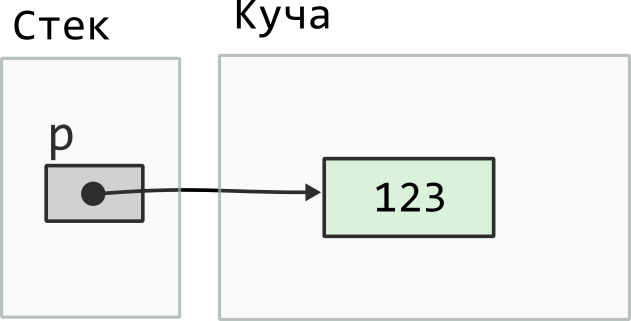
\includegraphics[scale=\mallocImagesScale]{../images/malloc_homework/00heap_size_t.png}
\end{center}


\item Строка (массив из элементов типа \texttt{char}).
\begin{center}
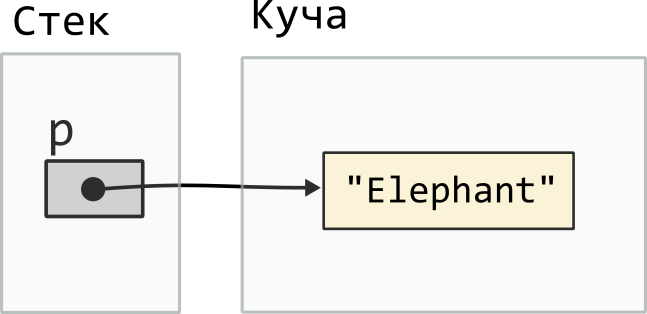
\includegraphics[scale=\mallocImagesScale]{../images/malloc_homework/01heap_char_array.png}
\end{center}

\item Указатель, указывающий на строку.
\begin{center}
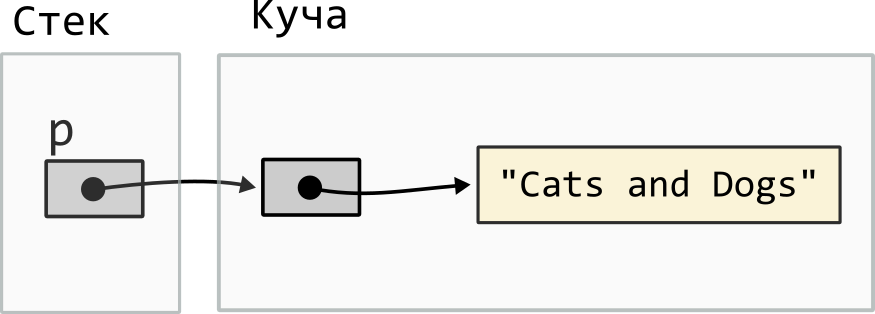
\includegraphics[scale=\mallocImagesScale]{../images/malloc_homework/02heap_pointer_char_array.png}
\end{center}


\item Структура типа \texttt{Book} из семинара про структуры. Для печати такой структуры можете использовать функцию \texttt{print\_book} из семинара про структуры.
\begin{lstlisting}
struct book 
{
    char title[50];
    int pages;
    float price;
};
typedef struct book Book;
\end{lstlisting}
\begin{center}
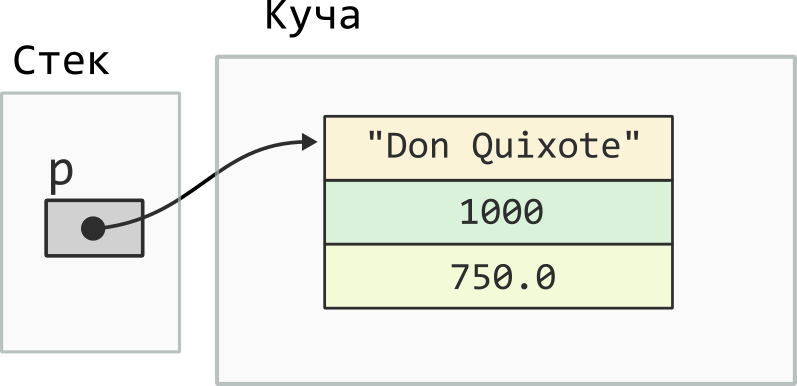
\includegraphics[scale=\mallocImagesScale]{../images/malloc_homework/03heap_struct_book.png}
\end{center}

\newpage
\item Указатель, указывающий на структуру на стеке.
\begin{center}
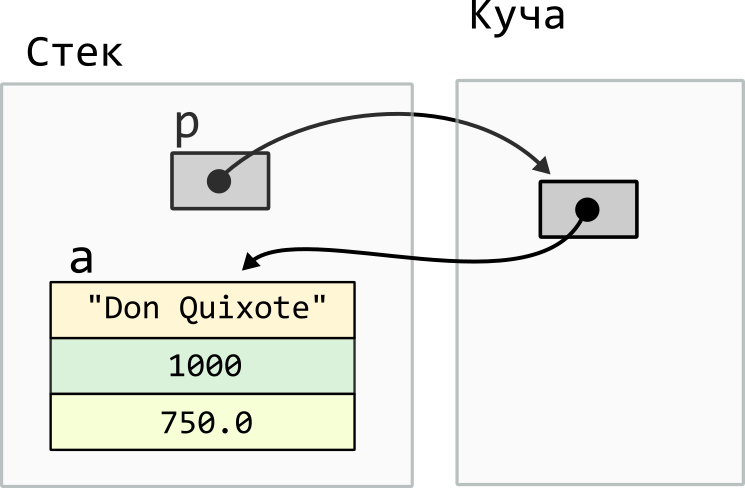
\includegraphics[scale=\mallocImagesScale]{../images/malloc_homework/04heap_pointer_stack_struct_book.png}
\end{center}


\item Указатель, указывающий на структуру в куче.
\begin{center}
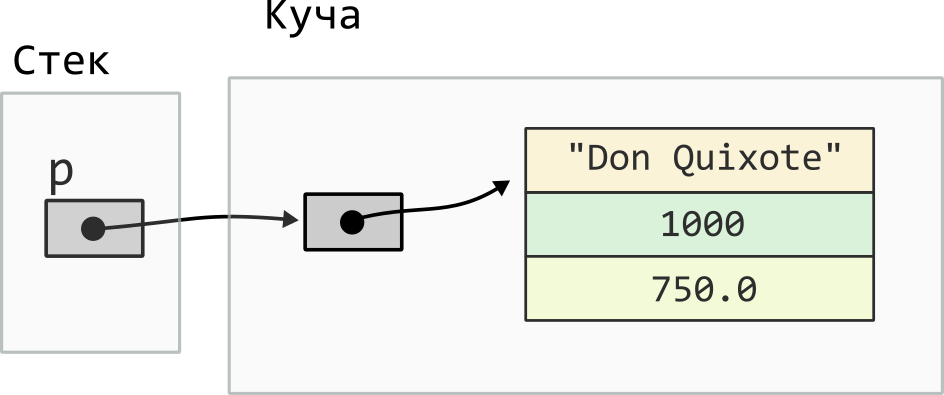
\includegraphics[scale=\mallocImagesScale]{../images/malloc_homework/05heap_pointer_struct_book.png}
\end{center}


\item Массив структур.
\begin{center}
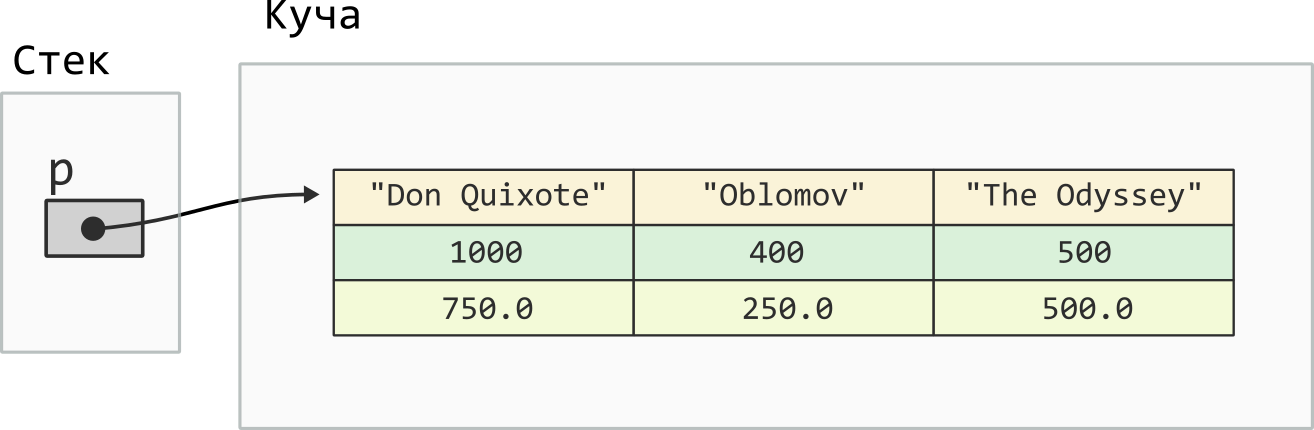
\includegraphics[scale=\mallocImagesScale]{../images/malloc_homework/06heap_struct_book_array.png}
\end{center}

\item Видоизмените структуру \texttt{Book}, чтобы она, вместо строки, хранила указатель на строку в куче. Таким образом у нас не будет ограничения на длину названия. Создайте такую структуру в куче. Функцию \texttt{print\_book} для такой структуры потребуется немного изменить.
\begin{lstlisting}
struct book 
{
    char* title;
    int pages;
    float price;
};
typedef struct book Book;
\end{lstlisting}

\begin{center}
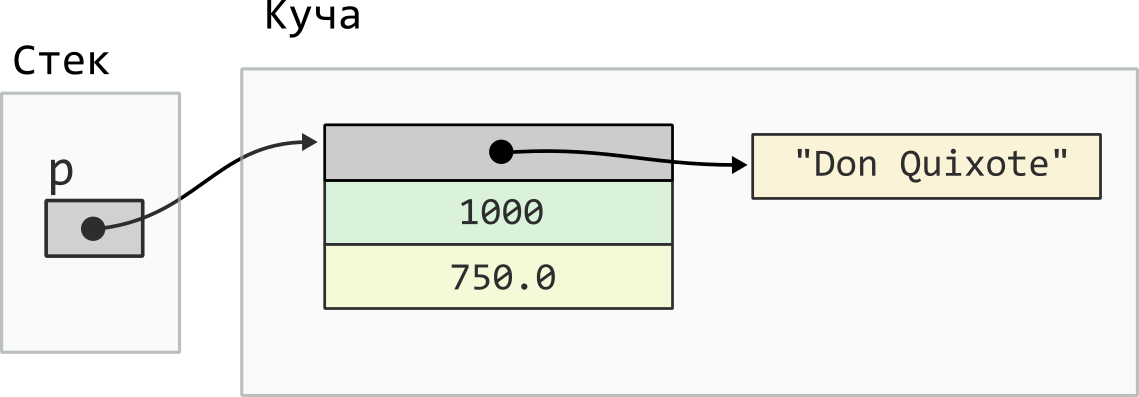
\includegraphics[scale=\mallocImagesScale]{../images/malloc_homework/07heap_struct_book_title_heap.png}
\end{center}

\item Массив таких структур в куче.
\begin{center}
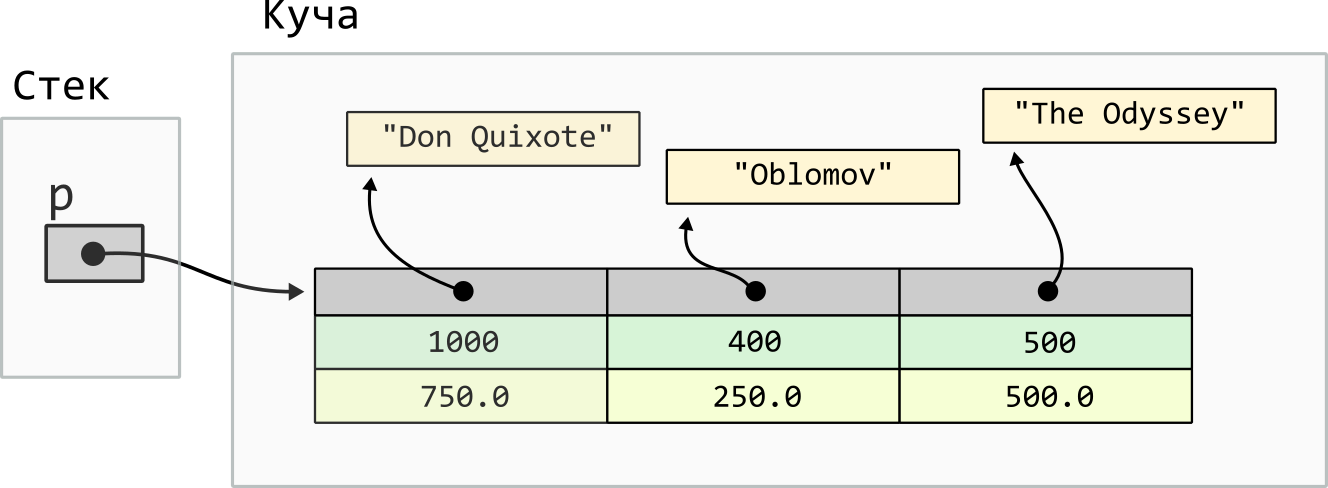
\includegraphics[scale=\mallocImagesScale]{../images/malloc_homework/08heap_array_struct_book_title_heap.png}
\end{center}


\item Создадим структуру \texttt{Library}, которая сможет хранить информацию о произвольном количестве книг.
\begin{lstlisting}
struct library 
{
    Book* books;
    int number_of_books;
};
typedef struct library Library;
\end{lstlisting}

\begin{center}
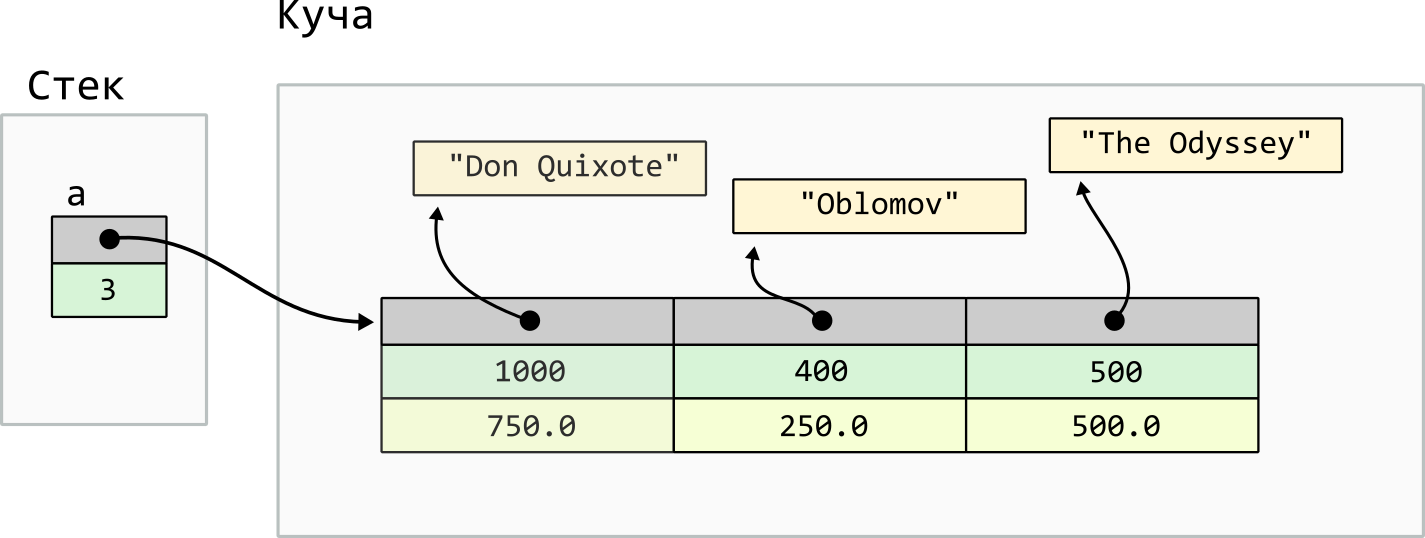
\includegraphics[scale=\mallocImagesScale]{../images/malloc_homework/09stack_struct_book_library.png}
\end{center}

Напишите функции для удобной работы с такой структурой:
\begin{itemize}
\item \texttt{library\_create} - функция должна задавать поля \texttt{books} и \texttt{number\_of\_books} структуры \texttt{Library}. При этом данная функция должна выделять необходимое количество памяти.
\item \texttt{library\_set} - должна задавать значение \texttt{i}-й книги.
\item \texttt{library\_get} - принимает на вход индекс \texttt{i} и возвращает указатель на \texttt{i}-ю книгу.
\item \texttt{library\_print} - должна печатать все книги библиотеки на экран.
\item \texttt{library\_destroy} - должна освобождать всю память и устанавливать значения полей в \texttt{NULL} и \texttt{0} соответственно.
\end{itemize}
\begin{lstlisting}
Library a;
library_create(&a, 3);
library_set(a, 0, "Don Quixote", 1000, 750.0);
library_set(a, 1, "Oblomov", 400, 250.0);
library_set(a, 2, "The Odyssey", 500, 500.0);
library_print(a);
print_book(library_get(a, 1));
library_destroy(&a);
\end{lstlisting}

Обратите внимание, что функции \texttt{library\_create} и \texttt{library\_destroy} должны принимать указатель на структуру \texttt{Library} так как они должны менять поля этой структуры.


\item Изменим структуру \texttt{Library} так, чтобы она хранила указатель на массив из указателей на структуры.
\begin{lstlisting}
struct library 
{
    Book** books;
    int number_of_books;
};
typedef struct library Library;
\end{lstlisting}

\begin{center}
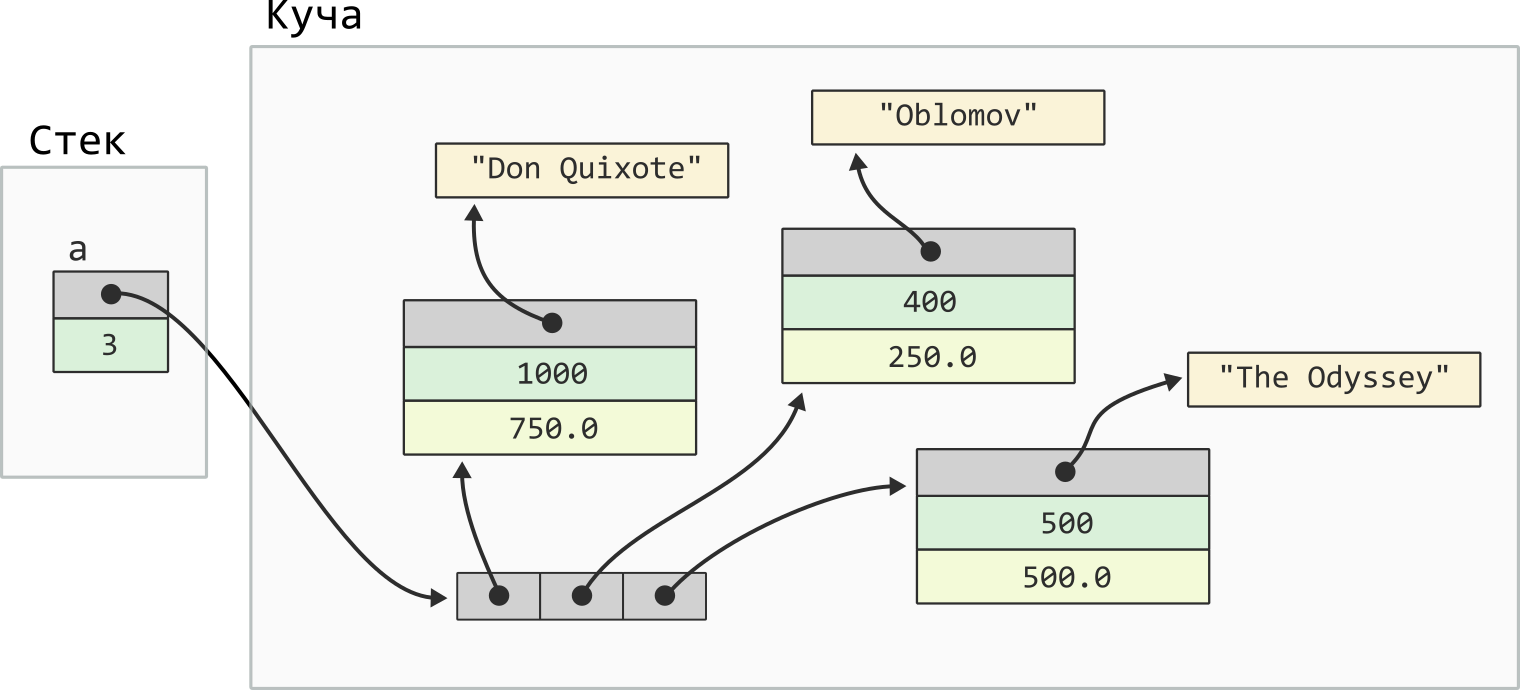
\includegraphics[scale=\mallocImagesScale]{../images/malloc_homework/11stack_struct_book_library.png}
\end{center}


Напишите функции для удобной работы с такой структурой:
\begin{itemize}
\item \texttt{library\_create} - функция должна задавать поля \texttt{books} и \texttt{number\_of\_books} структуры \texttt{Library}. При этом данная функция должна выделять память под массив из указателей и задавать все значения элементов массива значением \texttt{NULL}.
\item \texttt{library\_set} - должна задавать значение \texttt{i}-й книги.
\item \texttt{library\_get} - принимает на вход индекс \texttt{i} и возвращает указатель на \texttt{i}-ю книгу. Если структура с таким индексом ещё не создана, то функция должна вернуть \texttt{NULL}.
\item \texttt{library\_print} - должна печатать все книги библиотеки на экран.
\item \texttt{library\_destroy} - должна освобождать всю память (память под структуры и память под массив указателей) и устанавливать значения полей в \texttt{NULL} и \texttt{0} соответственно.
\end{itemize}

Работа с такой структурой не должна отличаться от работы со структурой из предыдущей подзадачи:
\begin{lstlisting}
Library a;
library_create(&a, 3);
library_set(a, 0, "Don Quixote", 1000, 750.0);
library_set(a, 1, "Oblomov", 400, 250.0);
library_set(a, 2, "The Odyssey", 500, 500.0);
library_print(a);
print_book(library_get(a, 1));
library_destroy(&a);
\end{lstlisting}

\end{enumerate}
\subsection{Геометрическая прогрессия}
Напишите функцию \texttt{float* get\_geometric\_progression(float a, float r, int n)}, которая возвращает указатель на динамический массив, содержащий геометрическую прогрессию из $n$ чисел: 
$a, ar, ar^2, ...$\\
Память должна выделяться динамически. Вызовите эту функцию из \texttt{main} и напечатайте первые 10 степеней тройки.


\newpage
\subsection{Динамический массив строк}
Динамический массив строк -- это двумерный динамический массив элементов типа \texttt{char}. 
Но с одной особеностью: размер строки задаётся не числом в отдельной переменной, а специальным нулевым символом на конце строки. Поэтому мы можем не хранить размер каждой строки. \\
Мы можем хранить количество строк в таком массиве в отдельной переменной, а можем просто выделить в массиве указателей на один элемент больше и хранить в этом элементе значение \texttt{NULL}. Таким образом мы можем найти количество строк в массиве.\\


\begin{center}
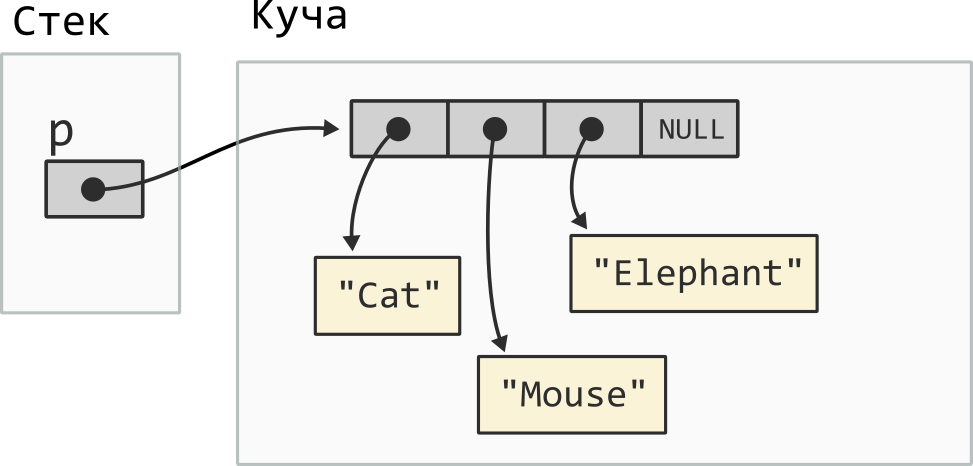
\includegraphics[scale=0.8]{../images/malloc_homework/12string_array_heap.png}
\end{center}

\begin{enumerate}
\item Написать функцию \texttt{char** get\_test\_strings()} который будет создавать массив строк, представленный на рисунке выше, и возвращать его.

\item Написать функцию \texttt{void print\_strings(FILE* stream, char** string\_array)} который будет печатать переданный массив строк \texttt{string\_array} в поток \texttt{stream}. С помощью этой функции напечатайте массив строк, представленный на рисунке, на экран.

\item Написать функцию \texttt{char** load\_lines(const char* filename)},
которая будет создавать динамический массив строк, считывать из файла все строки в этот массив строк, и возвращать его. Один из способов как это можно сделать:
\begin{itemize}
\item Пройдите по файлу с помощью \texttt{fgetc} и посчитайте количество строк в файле (количество \texttt{\textbackslash n} + 1).
\item Выделите необходимую память в куче под массив указателей (учтите нулевой указатель в конце).
\item Вернитесь в начало файла с помощью \texttt{fseek}.
\item Пройдите файл заново и считайте количество символов в каждой строке. Эту информацию нужно где-то хранить, поэтому выделите в куче временный массив в котором будет храниться длина каждой строки.
\item Выделите необходимую память для каждой строки (учтите нулевой символ в конце строк).
\item Вернитесь в начало файла с помощью \texttt{fseek}.
\item Пройдите файл заново и считайте каждую строку из файла в соответствующее место в массиве строк.
\item Освободите память под временный массив, закройте файл и верните из функции динамический массив строк.
\end{itemize}

\item Написать функцию \texttt{void destroy\_strings(char*** p\_string\_array)}, которая будет уничтожать динамический массив строк. Эта функция должна освобождать всю память (память под каждую строку и память под массив указателей). Также эта функция должна присваивать указателю \texttt{p} значение \texttt{NULL}.
\begin{lstlisting}
char** p = load_lines("three_little_pigs.txt");
destroy_strings(&p);
\end{lstlisting}

\item Написать функцию \texttt{void sort\_strings(char** words)}, которая будет сортировать все строки по алфавиту. Используйте функцию \texttt{strcmp}.
\end{enumerate}

\subsection{Сортировщик строк}
Напишите программу \texttt{line\_sorter}, которая будет считывать текстовый файл, сортировать строки этого файла по алфавиту и записывать результат в другой файл. Названия файлов функция должна принимать через аргументы командной строки.
Пример использования такой программы:

\begin{verbatim}
./line_sorter invisible_man.txt result.txt
\end{verbatim}

\end{document}
